%%% LaTeX Template: Article/Thesis/etc. with colored headings and special fonts
%%%
%%% Source: http://www.howtotex.com/
%%% Feel free to distribute this template, but please keep to referal to http://www.howtotex.com/ here.
%%% February 2011
%%%
%%% Modified October 2015 by CDM

%%%  Preamble
\documentclass[11pt,letterpaper]{article}
\usepackage[margin=1.0in]{geometry}
\usepackage[T1]{fontenc}
\usepackage[bitstream-charter]{mathdesign}
\usepackage[latin1]{inputenc}
\usepackage{amsmath}
\usepackage{xcolor}
\usepackage{cite}
\usepackage{hyphenat}
\usepackage{graphicx}
\usepackage{float}
\usepackage{subfigure}
\usepackage{sectsty}
\usepackage[compact]{titlesec}
\usepackage[tablegrid]{vhistory}
\allsectionsfont{\color{accentcolor}\scshape\selectfont}

%%% Definitions
\definecolor{accentcolor}{rgb}{0.0,0.0,0.5}
\newcommand{\teamname}{A-Team}
\newcommand{\productname}{Fiducial Career Display}
\newcommand{\coursename}{CSE 4316: Senior Design I}
\newcommand{\semester}{Summer 2016}
\newcommand{\docname}{System Requirements Specification}
\newcommand{\department}{Department of Computer Science \& Engineering}
\newcommand{\university}{The University of Texas at Arlington}
\newcommand{\authors}{Micah Dumont \\ Son Chau \\ Phat Tran \\ Bhakti Chhetri \\ Andy Wong}

%%% Headers and footers
\usepackage{fancyhdr}
	\pagestyle{fancy}						% Enabling the custom headers/footers
\usepackage{lastpage}
	% Header (empty)
	\lhead{}
	\chead{}
	\rhead{}
	% Footer
	\lfoot{\footnotesize \teamname \ - \semester}
	\cfoot{}
	\rfoot{\footnotesize page \thepage\ of \pageref{LastPage}}	% "Page 1 of 2"
	\renewcommand{\headrulewidth}{0.0pt}
	\renewcommand{\footrulewidth}{0.4pt}

%%% Change the abstract environment
\usepackage[runin]{abstract}			% runin option for a run-in title
%\setlength\absleftindent{30pt}			% left margin
%\setlength\absrightindent{30pt}		% right margin
\abslabeldelim{\quad}
\setlength{\abstitleskip}{-10pt}
\renewcommand{\abstractname}{}
\renewcommand{\abstracttextfont}{\color{accentcolor} \small \slshape}	% slanted text

%%% Start of the document
\begin{document}

%%% Cover sheet
{\centering \huge \color{accentcolor} \sc \textbf{\department \\ \university} \par}
\vspace{1 in}
{\centering \huge \color{accentcolor} \sc \textbf{\docname \\ \coursename \\ \semester} \par}
\vspace{0.5 in}
\begin{figure}[h!]
	\centering
   	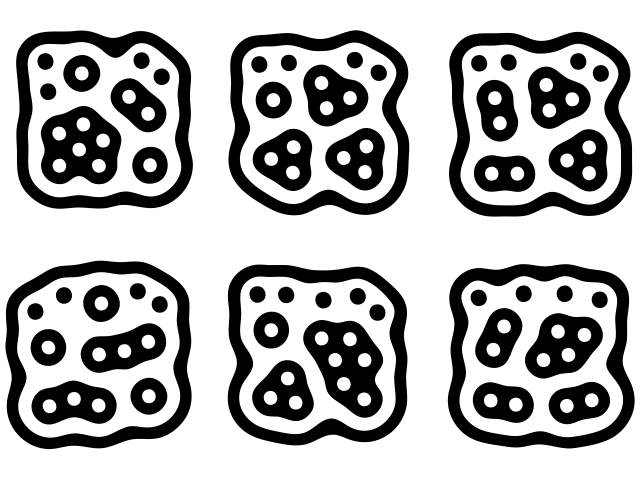
\includegraphics[width=0.60\textwidth]{images/reactivision02}
\end{figure}
\vspace{0.5 in}
{\centering \huge \color{accentcolor} \sc \textbf{\teamname \\ \productname} \par}
\vspace{0.5 in}
{\centering \large \sc \textbf{\authors} \par}
\newpage


%\vspace{1 in}
%\centerline{January 13th, 2012}
%\newpage

%%% Revision History
\begin{versionhistory}
  	\vhEntry{0.1}{07.22.2016}{MD}{document creation}
\end{versionhistory}
\newpage

%%% Table of contents
\setcounter{tocdepth}{2}
\tableofcontents
\newpage

%%% List of figures and tables (optional)
\listoffigures
%\listoftables
\newpage

\section{Product Concept}
This section describes the purpose, use and intended user audience for the Fiducial Career Display.
The purpose of this  project is to build a top flat surface table with that  provides user interface with needed information. The system consists of fiducial markers which will be placed on top of the surface of the table and will be able to move around the surface.

\subsection{Purpose and Use}
This product is meant to replace the iPad career wall in the Air Force Performance Lab. Each fiducial markers will display a career available in the Air Force. When the marker is placed on the table, an interface will appear to allow the user to page through different details about that career. Any user can walk up and pick up a maker and start interacting to explore the career description.Their objective is to change people\'s perceptions about what the Air Force does and inspire them to learn more while generating qualified leads.
\subsection{Intended Audience}
The intended audiences of stakeholders for this specification of the project include:
Recruitment officer, who can show the information for intended audience
The visitor, normal people who interested in the Air Force careers can look into it and find the materials they need

This product was designed specifically for the Air Force Performance Lab, but it can be repurposed to other commercial uses such as museums, trade shows and so on...
\begin{figure}[h!]
	\centering
   	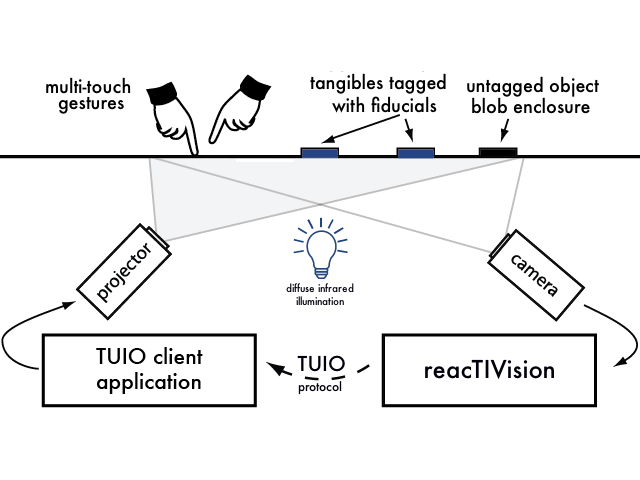
\includegraphics[width=1\textwidth]{images/reactivision03}
    \caption{X conceptual drawing}
\end{figure}

\newpage
\section{Product Description}
This section provides an overview of the Fiducial Career Display. A table will be constructed upon which the top surface will consist of a video display. The display will recognize specific objects played on top of it and will be able to track their movement across the surface if moved or rotated. Object recognition will be dependent on uniquely shaped or patterned markers placed on the bottom of the object. For objects placed on the surface of the table that do not contain a recognized pattern (like a fingertip), the table will treat as user interaction (touch gesture). Each marker will display the details including text, image, or videos about that career.
\subsection{Features \& Functions}
Hardware features:
\begin{itemize}
\item A semi-transparent acrylic board that make the table top as well as interactive display.
\item An infrared camera used to capture the input from the user.
\item A short throw projector mounted below the table to provide the interactive display.
\item A computer to run the recognition and application softwares.
\item A Fiducial marker that will represent a career. When a marker is placed on the table, an interface will appear to allow the user to page through different details about that career.
\end{itemize}


Software Features:
\begin{itemize}
\item Movable modular interface.
\item Automatic orientation based on position on table.
\item Navigable content.
\item Logo screen when not engaged.
\item Transitions in and out when marker is introduced and removed.
\item Track type of markers on the table.
\end{itemize}

\subsection{External Inputs \& Outputs}

\begin{table}[H]
\centering
\caption{Input \& Output}
\label{input}
\begin{tabular}{|l|l|l|}
\hline
Name            & Description                                                                                                              & Use                                                                                                      \\ \hline
Input           &                                                                                                                          &                                                                                                          \\ \hline
Fiducial Marker & \begin{tabular}[c]{@{}l@{}}Fiducial markers which can be tracked from \\ a camera and interpreted using software.\end{tabular} & \begin{tabular}[c]{@{}l@{}}Place on top of the table for \\ activating career choice menu\end{tabular} \\ \hline
Finger touch    & Human finger on the table surface                                                                                        & \begin{tabular}[c]{@{}l@{}}Use to select and interact\\ with the menu\end{tabular}                   \\ \hline
Output          &                                                                                                                          &                                                                                                          \\ \hline
Display         & \begin{tabular}[c]{@{}l@{}}A semi-transparent tabletop capable \\ of display\end{tabular}                              & \begin{tabular}[c]{@{}l@{}}Projected the screen to the \\ table surface\end{tabular}                    \\ \hline
Sound           & Audio source                                                                                                             & Play on input and media request                                                                                  \\ \hline
\end{tabular}
\end{table}

\subsection{Product Interfaces}

\begin{figure}[H]
	\centering
   	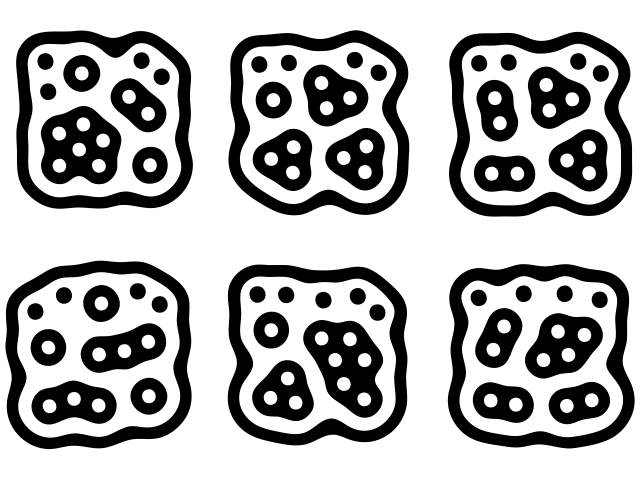
\includegraphics[width=0.6\textwidth]{images/reactivision02}
    \caption{Fiducial pattern examples}
\end{figure}

\begin{figure}[H]
	\centering
   	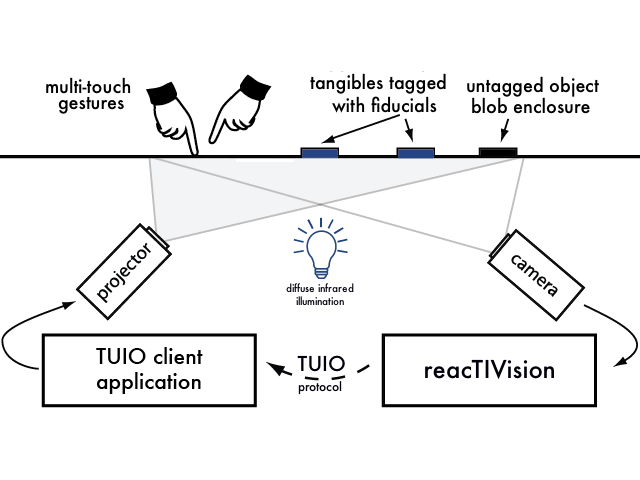
\includegraphics[width=0.9\textwidth]{images/reactivision03}
    \caption{Table concept }
\end{figure}

\begin{figure}[H]
	\centering
   	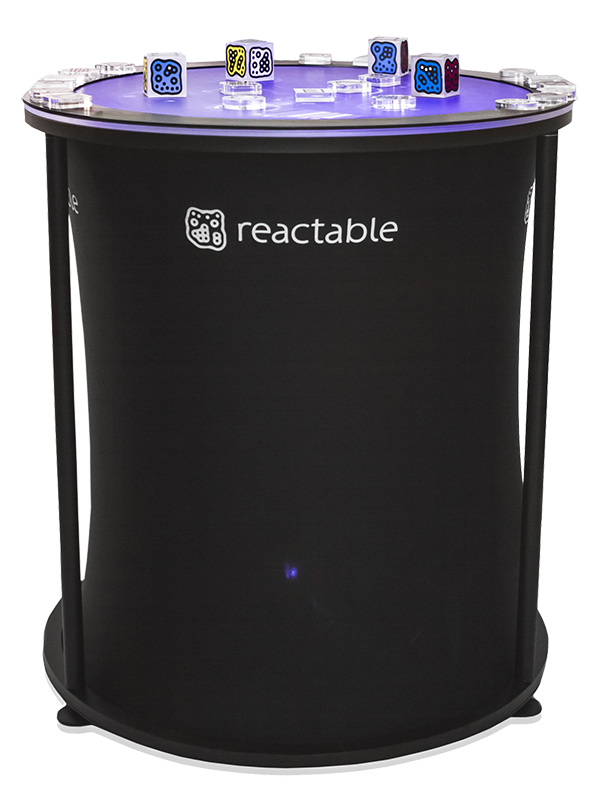
\includegraphics[width=0.4\textwidth]{images/ReacTable-live-6-instrument}
    \caption{Round table concept}
\end{figure}

\begin{figure}[H]
	\centering
   	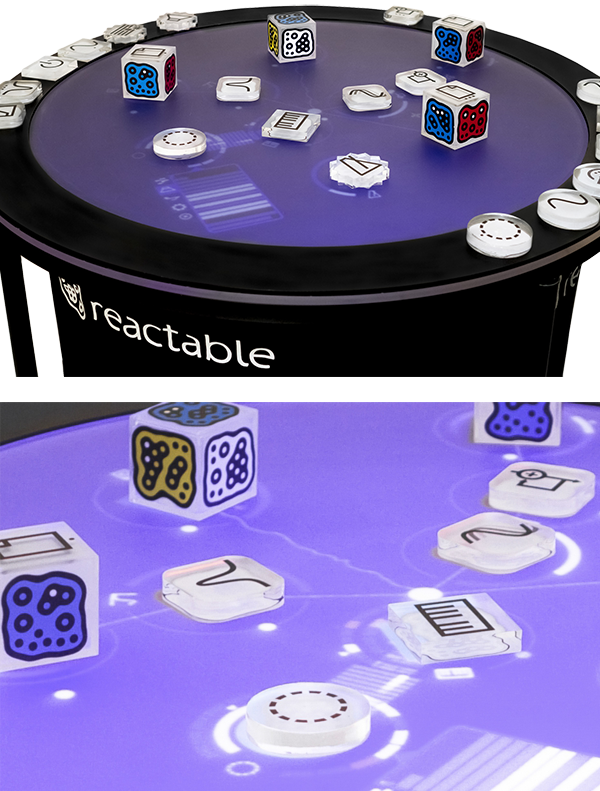
\includegraphics[width=0.5\textwidth]{images/ReacTable-instrument-detail1}
    \caption{Round table concept \cite{concept2}}
\end{figure}

\newpage
\section{Customer Requirements}
For this project, a table will be constructed upon which the top surface will consist of a video display.
The display will recognize specific objects played on top of it and will be able to track their
movement across the surface if moved or rotated. Object recognition will be dependent on
uniquely shaped or patterned markers placed on the bottom of the object. For objects placed on
the surface of the table that do not contain a recognized pattern (like a fingertip), the table will
treat as user interaction (touch gesture).

\subsection{The product will be a table of three feet by three feet in any geometric shape that is feasible}
\subsubsection{Description}
While geometric shape isn't important, the table should be tall enough for items to be placed on it without being obscured. 
\subsubsection{Source}
Paul Medcalf (Customer)
\subsubsection{Constraints}
The projector must be able to project evenly onto the surface and have a focal length that allows the display to remain in focus. The resulting structure should be stable enough to support several aluminum cylinders in the worst case.
\subsubsection{Standards}
NA
\subsubsection{Priority}
Critical

\subsection{The product will recognize user touch interaction}
\subsubsection{Description}
Utilizing a projector and sensor, the table will recognize all input that is not a fiducial markers as touch input.
\subsubsection{Source}
Paul Medcalf (Customer)
\subsubsection{Constraints}
High precision may not be possible due to sensor limits and input lag.
\subsubsection{Standards}
NA
\subsubsection{Priority}
High

\subsection{The product will recognize fiducial markers}
\subsubsection{Description}
Utilizing the a fiducial recognition library, the table will recognize the fidcuial markers of multiple different career cylinders or pucks to display career information.
\subsubsection{Source}
Paul Medcalf (Customer)
\subsubsection{Constraints}
May be limitations depending on the fiducial recognition library used and the projection surface utilized.
\subsubsection{Standards}
NA
\subsubsection{Priority}
Critical

\subsection{The product will display career information}
\subsubsection{Description}
The product will maintain a database of career information, which will trigger a view operation upon placement of a marker.
\subsubsection{Source}
Paul Medcalf (Customer)
\subsubsection{Constraints}
The storage capacity of the device will determine the limit to the number of entries.
\subsubsection{Standards}
NA
\subsubsection{Priority}
Critical

\subsection{The product will allow modification of the career information}
\subsubsection{Description}
A content management system will be created to update career entries, delete them, and add new ones.
\subsubsection{Source}
Micah Dumont
\subsubsection{Constraints}
The User Interface may be difficult to type with, so a keyboard may be necessary for input. This content management system may consist of directly querying the database if time constraints become a factor.
\subsubsection{Standards}
NA
\subsubsection{Priority}
Medium

\subsection{The product will utilize a dial interface}
\subsubsection{Description}
The final product will allow rotation of the fiducial markers to affect user interaction in a meaningful way. For example, to access different froms of media within a particular career.
\subsubsection{Source}
Micah Dumont
\subsubsection{Constraints}
The detection hardware might make this particular implementation difficult. This will need to be allowed by the Reactivision Library, or the Fiducial Library in use.
\subsubsection{Standards}
NA
\subsubsection{Priority}
Medium

\subsection{The product will have a modern user interface}
\subsubsection{Description}
The animations used in the project's user interface will be intuitive and easy for users to learn.
\subsubsection{Source}
Micah Dumont
\subsubsection{Constraints}
None
\subsubsection{Standards}
NA
\subsubsection{Priority}
Medium

\newpage
\section{Packaging Requirements}
The following are the packaging requirements for the Tangible User Interface Table project.

\subsection{The product will be self-contained to the extent that it can be transported easily}
\subsubsection{Description}
The construction of the table will be sturdy enough to allow movement from one location to another by loading it into a truck.
\subsubsection{Source}
Micah Dumont
\subsubsection{Constraints}
Not a guarantee that the final product will be modular, but it will be sturdy.
\subsubsection{Standards}
NA
\subsubsection{Priority}
High

\subsection{The product's user interface will be pre-loaded}
\subsubsection{Description}
The user interface for the device will be pre-loaded onto the device, and possibly backed up onto a flash drive for the end user to reinstall if needed.
\subsubsection{Source}
Micah Dumont
\subsubsection{Constraints}
Budgetary constraints may prevent the backup option.
\subsubsection{Standards}
NA
\subsubsection{Priority}
High

\subsection{The product components will be securely mounted}
\subsubsection{Description}
The projector, sensors, lights, and other components will be securely mounted to the inside of the table to prevent shifting during transport.
\subsubsection{Source}
Micah Dumont
\subsubsection{Constraints}
Need sufficient room inside the enclosure for components to be mounted.
\subsubsection{Standards}
NA
\subsubsection{Priority}
High

\subsection{The final product will come with career cylinders}
\subsubsection{Description}
The final product will have 5-10 cylinders or pucks, each of which displays a different career for the United States Airforce, with information provided from the U.S. Airforce Website.
\subsubsection{Source}
Micah Dumont
\subsubsection{Constraints}
The geometrical shape of the markers is subject to change for visibility purposes.
\subsubsection{Standards}
NA
\subsubsection{Priority}
High

\subsection{The product will have an enclosure}
\subsubsection{Description}
All non-interactive components of the project will be conceiled within an enclosure that avoids distracting the user with unnecesary interactions.
\subsubsection{Source}
Micah Dumont
\subsubsection{Constraints}
None
\subsubsection{Standards}
NA
\subsubsection{Priority}
Medium

\subsection{The product will come with all necessary accessories}
\subsubsection{Description}
The product will include all wires, power supplies, operating systems, software CDs, etc in order to ensure proper operation.
\subsubsection{Source}
Micah Dumont
\subsubsection{Constraints}
None
\subsubsection{Standards}
NA
\subsubsection{Priority}
Critical

\newpage
\section{Performance Requirements}
Include a header paragraph specific to your product here. Performance requirements address items such as: how fast specific critical operations must complete; how long it takes to start/stop activities; how long the battery must last; maximum time it must take to set up; etc.

\subsection{Run smoothly during usage }
\subsubsection{Description}
Detailed requirement description...
\subsubsection{Source}
Source
\subsubsection{Constraints}
Detailed description of applicable constraints...
\subsubsection{Standards}
List of applicable standards
\subsubsection{Priority}
Priority

\subsection{Respond to the user input quickly }
\subsubsection{Description}
Detailed requirement description...
\subsubsection{Source}
Source
\subsubsection{Constraints}
Detailed description of applicable constraints...
\subsubsection{Standards}
List of applicable standards
\subsubsection{Priority}
Priority

\subsection{Power up and shut down upon user activation }
\subsubsection{Description}
Detailed requirement description...
\subsubsection{Source}
Source
\subsubsection{Constraints}
Detailed description of applicable constraints...
\subsubsection{Standards}
List of applicable standards
\subsubsection{Priority}
Priority

\newpage
\section{Safety Requirements}
Include a header paragraph specific to your product here. Safety requirements might address items specific to your product such as: no exposure to toxic chemicals; lack of sharp edges that could harm a user; no breakable glass in the enclosure; no direct eye exposure to infrared/laser beams; packaging/grounding of electrical connections to avoid shock; etc.

\subsection{The system shall draw power from power supply  }
\subsubsection{Description}
The projector system will take in power from a nearby safety plug.
\subsubsection{Source}
Development Team
\subsubsection{Constraints}
Safety plug limits the electrical intake of the plug.
\subsubsection{Standards}
NA
\subsubsection{Priority}
High

\subsection{The system shall be safe for a user to handle and input commands }
\subsubsection{Description}
The table will be neatly organized and easy to interact with, wires will be hidden and kept away to avoid injuring the user.
\subsubsection{Source}
Development Team
\subsubsection{Constraints}
The space available and structure will limit how much can be done to the product.
\subsubsection{Standards}
NA
\subsubsection{Priority}
High

\subsection{The system shall be stable and hold its structure }
\subsubsection{Description}
The table will be able to support weight and be sturdy enough to not break.
\subsubsection{Source}
Development Team
\subsubsection{Constraints}
The supporting structure will only support as much weight as the materials will hold. 
\subsubsection{Standards}
NA
\subsubsection{Priority}
High

\subsection{The fiducial markers shall be safe for the user to handle and interact with the table }
\subsubsection{Description}
The cylinders with the fiducial markers will be made of safe material for any user to handle.
\subsubsection{Source}
Development Team
\subsubsection{Constraints}
Material for the fiducial marker constrains this requirement.
\subsubsection{Standards}
NA
\subsubsection{Priority}
High

\subsection{The projector shall be placed appropiately to project only onto the table surface }
\subsubsection{Description}
The projector will project onto the table surface which will absorb some of the light to prevent exposure to the eyes.
\subsubsection{Source}
Development Team
\subsubsection{Constraints}
The table top will have a spray to insulate light. The coating may not block out all light.
\subsubsection{Standards}
NA
\subsubsection{Priority}
High

\subsection{The table shall be standard table height for easy user interaction }
\subsubsection{Description}
The table will be standard table height to allow users of all heights to easily interact with.
\subsubsection{Source}
Development Team
\subsubsection{Constraints}
Will be dependent on throw distance of projector.
\subsubsection{Standards}
NA
\subsubsection{Priority}
High

\subsection{The table shall be able to fit through a standard doorway }
\subsubsection{Description}
The table must be kept in a size that allows for movement in and out doorways.
\subsubsection{Source}
Development Team
\subsubsection{Constraints}
Doorway size affects this requirement and the size of the table.
\subsubsection{Standards}
NA
\subsubsection{Priority}
High

\subsection{The system shall not exceed the highest operating temperature of the components }
\subsubsection{Description}
The table must be kept with in a temperature range for the sensor and projector to remain operational. 
\subsubsection{Source}
Development Team and Component Providers
\subsubsection{Constraints}
Projector and sensor as well as material of the table limit temperature.
\subsubsection{Standards}
NA
\subsubsection{Priority}
High

\newpage
\section{Maintenance \& Support Requirements}
This section of System Requirement Specification includes the list and description of Maintenance and Support Requirements for the project. This section provides all necessary information about how to setup product and do necessary maintenance after the product delivery. This section includes list of requirement such as user manual which describes how to use the product and troubleshooting guide which explains how run troubleshoot for minor problems and all other necessary tools and supports that are required for the users to operate the product smoothly. 

\subsection{User Manual}
\subsubsection{Description}
Product shall be delivered with a convenient and easy to follow user manual. User manual provide guidelines how to use the product. User manual includes table of content which provide user with a convenient way to get to the specific part of the manual using the page numbers. It also includes system overview section which explains about the product; getting started section which explains initial steps how to set up the system and make it ready to use. There will be a section for each major component of the product with explicit instructions. End of the manual includes Glossary which provides definition of technical terms used on the manual. 
\subsubsection{Source}
Team
\subsubsection{Constraints}
User manual will be written in English language. Manual won't be available in any other language except English. 
\subsubsection{Standards}
Standard American English
\subsubsection{Priority}
Moderate

\subsection{Source Code}
\subsubsection{Description}
Source code shall be available to the customer on the final delivery. Source code will be well commented making it easily readable. Each functionality on the source code will be made simple and logical as possible using comments. 
\subsubsection{Source}
Team 
\subsubsection{Constraints}
None
\subsubsection{Standards}
None
\subsubsection{Priority}
High

\subsection{Documentation Availability}
\subsubsection{Description}
Documentation done throughout the development phase of this project shall be included on the final delivery of this product. This documentation will be handy for customers give ideas how the system is build. Documentations includes Project Charter, System Requirements Specification, Architectural Design Specifications, Detailed Design Specifications, and System Test Plan. Documentation will be well formatted and schematics which makes it easy to understand. 
\subsubsection{Source}
Team
\subsubsection{Constraints}
None
\subsubsection{Standards}
Standard American English
\subsubsection{Priority}
Moderate

\subsection{Troubleshooting Guide}
\subsubsection{Description}
System troubleshooting guide shall be available to the customer on the final delivery of the product. Troubleshooting guide will be easy to follow guidelines and assists users to detect the problems. Troubleshooting guide will be well formatted and schematics with symbolic presentation which provides the user a convenient way to detect the problem and eliminate potential causes.
\subsubsection{Source}
Team 
\subsubsection{Constraints}
Troubleshooting Guide will be written in English Language. It won't be available in any other language except English. 
\subsubsection{Standards}
Standard American English
\subsubsection{Priority}
High

\subsection{Projector Lamp Replacement}
\subsubsection{Description}
The project consists of different major hardware components. One of the most important hardware component is projector. Every projector comes with hours of life of lamp. When brightness start getting dimmer, it is a warning sign that lamp of projector needs to be replaced. Guidelines will be provided how to replace lamp on user manual. 
\subsubsection{Source}
Customer
\subsubsection{Constraints}
None
\subsubsection{Standards}
None
\subsubsection{Priority}
High

\subsection{Database Maintenance}
\subsubsection{Description}
MySQL database will be used for storing contents of the product. Developer Team will be responsible for creating and maintenance of database throughout the development phase of the product and Customer will be responsible for database maintenance after product delivery. 
\subsubsection{Source}
Customer
\subsubsection{Constraints}
None
\subsubsection{Standards}
None
\subsubsection{Priority}
High

\subsection{Hardware Support and Maintenance}
\subsubsection{Description}
The product includes hardware components which needs to be inspected and tested with scheduled time period. Hardware components need to be replaced as necessary. User manual and troubleshooting guide can be referred for more detail information about the hardware components. 
\subsubsection{Source}
Customer
\subsubsection{Constraints}
None
\subsubsection{Standards}
None
\subsubsection{Priority}
Moderate

\subsection{Demonstration and Training}
\subsubsection{Description}
Training will be provided to the customer showing all the major functionality of the product. User manual can be used for further future references. 
\subsubsection{Source}
Team
\subsubsection{Constraints}
None
\subsubsection{Standards}
None
\subsubsection{Priority}
Moderate


\newpage
\section{Other Requirements}
This section of System Requirement Specification describes the requirements that are not included in any of the other requirement categories. 

\subsection{American English Written Standard for Documentation}
\subsubsection{Description}
All the necessary documentation for the project shall be done in Standard American English. 
\subsubsection{Source}
Team
\subsubsection{Constraints}
None
\subsubsection{Standards}
Standard American English
\subsubsection{Priority}
Moderate

\newpage
\section{Future Items}
In this last section, you will reiterate all requirements that are listed as priority 5. This is repetitive, but necessary as a concise statement of features/functions that were considered/discussed and documented herein, but will NOT be addressed in the prototype version of the product due to constraints of budget, time, skills, technology, feasibility analysis, etc. Use the following format for this section.

\subsection{The system shall display content for all careers available in the Air Force}
\subsubsection{Description}
User can place a cylinder object on the surface. The table will recognize the object and show the content of each career. Each cylinder will represent a career in the Air Force.
\subsubsection{Source}
Client
\subsubsection{Constraints}
There are hundreds of careers available in the Air Force and have more later on. We need to collect all details about these careers and keep up with new careers.
\subsubsection{Standards}
The content for each career should contain the title, image, video, description and qualification summary.
\subsubsection{Priority}
High

\subsection{The display shall recognize fiducial markers and perform special features}
\subsubsection{Description}
The display shall orient automatically based on position on the table, movable modular interface and navigable content. 
\subsubsection{Source}
Client
\subsubsection{Constraints}
The information and content around marker take up most of the screen. It would be difficult to have multiple people interacting simultaneously.
\subsubsection{Standards}
NA
\subsubsection{Priority}
High

\subsection{The table shall design for profesional use}
\subsubsection{Description}
The table will be compact, solid and transportable in customer's desired custom design. The touch surface allows for strong and safe built quality, protected against scratches, fluids and vandalism.
\subsubsection{Source}
Development Team
\subsubsection{Constraints}
More experiments to obtain the proper material for the surface that it had to take considerable weight without flexing, diffuse infrared illumination for projection, and be robust to repeated use.
\subsubsection{Standards}
NA
\subsubsection{Priority}
High

\subsection{The delivery product shall be a perfect package}
\subsubsection{Description}
The product will be arrived fully assembled to customer. There is no need for installation technicians, nor any special set-up or requirements. The customer unpack it, plug it in, press the button and get started.
\subsubsection{Source}
Development Team
\subsubsection{Constraints}
NA
\subsubsection{Standards}
NA
\subsubsection{Priority}
High

\subsection{The surface shall process multiple touches, gesture }
\subsubsection{Description}
The surface will provide superior responsiveness and accuracy. The multitouch technology featured in the Platform tables will be the same reliable touch technology used in smart phones and tablets. Users can use hand and finger gestures to interact with multi-media content and pull on an image to zoom in and out.  
\subsubsection{Source}
Development Team
\subsubsection{Constraints}
NA
\subsubsection{Standards}
The surface should be water and dust resistant.
\subsubsection{Priority}
High

\subsection{The reacTIVision framework shall be improved and new features added }
\subsubsection{Description}
An important improvement in the next release will be the inclusion of the plain finger tracking layer which doesn't require fiducial stickers. We will include additional fiducials engines such as Barcodes, ARToolkit into reacTIVision.
\subsubsection{Source}
Development Team
\subsubsection{Constraints}
NA
\subsubsection{Standards}
NA
\subsubsection{Priority}
High

\subsection{The system shall have more advanced features }
\subsubsection{Description}
System will recognize other objects besides fiducial markers. For example, it will allow user create digital paintings with paintbrushes. User can place their smartphones on the surface, and the system will display the images in the phone's gallery.
\subsubsection{Source}
Development Team
\subsubsection{Constraints}
NA
\subsubsection{Standards}
NA
\subsubsection{Priority}
High

\newpage

%%% References
\bibliographystyle{plain}
\bibliographystyle{reference/IEEEtran_custom}
\bibliography{reference/refs}{}

\end{document}
